\chapter{Literature Review on Brain Data Modelling and Machine Learning}

\section{A Review on Modelling Brain Data}
The human curiosity to understand the neural activity associated with cognition and perception is as old as the field of neuroscience itself. During its inception, neuroscience studies were focused on invasive techniques for modelling the brain. This strand of research suffered from two major disadvantages:
\begin{enumerate}
	\item The studies were non-functional studies due to their invasive nature \citep{geschwind1974disconnexion, shallice1988neuropsychology}.
	\item These studies needed to be implemented on non-human subjects \citep{felleman1991distributed, pandya1985architecture} due to the risk associated with invasive procedures.
\end{enumerate}
Due to these limitations, therefore, for many years, neuroscientists faced great difficulties in measuring the neural activity in the mammalian brain, while they performed tasks or simply rested. The advent of non-invasive techniques, such as electrical activity (Electroencephalography, Electromyography, Electronystagmography), haemodynamic activity (fMRI), water diffusion (DTI), and others, allowed for indirect measurements of neural activity and connectivity, leading to the affordance of a new departure of computational neuroscience. 
\begin{itemize}
	\item Functional Magnetic Resonance Imaging (fMRI): Magnetic resonance imaging (MRI) applies an external magnetic field to align the magnetic moments of hydrogen ions in the body and then applies a radio frequency pulse, which flips the ions in the opposite direction. The recovery of these hydrogen ions back to the direction of the external magnetic field produces a current, which generates the black and white image in an MRI photo. Resting state functional magnetic resonance imaging (rs-fMRI) measures changes in blood oxygenation within the brain during rest. When neurons are activated in the brain, they expend energy, which needs to be replaced. This is achieved via an increase in blood flow to the active area (occurring between 6 and 10 seconds after activity is initiated). This increase in blood flow produces a net decrease in deoxygenated haemoglobin levels, changing the magnetic properties of the blood. Areas of high activity are consequently associated with higher signal in the MRI and this can be measured across time.
	\item Electroencephalography (EEG): EEG is a technique for measuring the electrical activity of the brain. Silver chloride electrodes placed on the scalp record the integrated activity of a large number of neurons within the brain. Only neural structures with a specific spatial organisation (\emph{i.e.}, layers of neurons with all cell bodies/dendrites facing in the same direction, such as the cortex, thalamus and cerebellum) can generate scalp potentials. Consequently, non-invasive EEG can only measure a subset of the overall activity of the brain. Despite this limitation, however, EEG is a valuable tool for investigating abnormalities in brain function and provides a useful data source for classifying patient populations with known changes in their EEG output.
	\item Diffusion Tensor Imaging (DTI): DTI measures the net movement of water within the brain. Water molecules outside of the cell have equal probability of movement in every direction. However, when water is trapped within a neuronal cell (within an axon or dendrite), its diffusion is restricted to movement along the direction of the axon or dendrite. The diffusion direction of these trapped water molecules can be measured using DTI, providing a map of neuronal tracts (white matter) within the brain.
	
\end{itemize}

Numerous studies have focused on analysing and modelling neural activities related to cognitive or non-cognitive tasks, using single modalities of non-invasive techniques, such as EEG, fMRI or DTI. Functional Magnetic Resonance (fMRI) was used by \citet{boksman20054} to study brain connectivity related to word fluency during the first episode of schizophrenia. \citet{supekar2008network} used fMRI to study brain connectivity in Alzheimers disease. Diffusion Tensor imaging (DTI) was also employed in the works of \citet{eluvathingal2006abnormal, price2007abnormal} for cognitive studies. \citet{ravan2015machine} used EEG data for studying the effect of Clozapine therapy in schizophrenia. \citet{cabeza2000imaging} studied fMRI and PET, two modalities of neuroimaging to explore the functional anatomy of different cognitive functions, such as, attention, perception, language and so on. \citet{mcclure2007fmri} studied a predictive model for treatment of anxiety disorder in young children. DTI is used by \citet{hamstra2007diffusion}, as a biomarker for treatment response in oncology. \citet{gordon2007integrating} discussed using neuromarkers like fMRI and DTI for brain-related personalised medicine and treatment. Apart from these, applications, such as, Brain Computer Interfaces (BCI), neuroprosthetics, neuro-rehabilitation are a few of many other areas, which can potentially gain from brain data modelling and analysis. 
All of the research work discussed above show the trend of modelling a single modality of brain data. This is primarily due to the technological constraints associated with simultaneous acquisition of multiple modalities of brain data. Concurrent recording suffers from several technical difficulties, such as, ballistocardiographic artefact, MRI pulse artefact and others, leading to high noise to signal ratio. Current technical advances in MRI and EEG recordings, though, have overcome the aforementioned difficulties and allow for simultaneous recording of mixed modalities of brain data \citep{menon2005combined, horovitz2002correlations}. This is ground breaking, as fused analysis of multiple data types is potentially more informative about the complex brain activity during the measured task. Until recently, the most commonly used method of integrated data analysis for this kind of problem was by converging evidence \citep{horwitz2002can}. Typically, each data type is analysed separately, and the results from other analyses that support one's finding are discussed in the discussion Section. A standard sentence looks like "the activation that was found in region X is consistent with studies in patients with focal lesion in region X and in ERP studies, where a latency in the Y component on task Z has been observed during.." \citep{horwitz2002can}. \citet{horwitz2002can} also discussed an alternative data fusion analysis called computational neural modelling. This is done by creating biologically realistic neural network models where each network simulates data of a certain type and is compared with observed data. One major setback of this paradigm of data analysis is that the hypothesis-driven neural network model is built under several assumptions for simulated data generation. Hence, it is difficult to know, whether any lack of agreement between observed and simulated data is due to the assumptions in the model, or whether it is simply wrong.

There is a third alternative for multi-modal data integration, known as direct data fusion \citep{george1995mapping}. Direct data fusion can be loosely defined as, the technique for directly fusing multiple datasets using statistical and machine learning algorithms. \citet{biessmann2011analysis} presented a detailed description and analysis of this approach. In this approach, if one is interested in the neural potentials induced by a certain stimulus event, one averages epochs of EEG time series aligned to the presentation of that stimulus. If one is not interested in the exact phase of the neural response, one often extracts the amplitude modulations of neural oscillations in a certain frequency band (e.g. \citep{laufs2006bold}). For fMRI data, one typically extracts patterns of activity that are correlated with the time course of the experimental stimulus. Several exploratory unsupervised methods are also proposed for fused data analysis. In \citep{eichele2008unmixing}, temporal ICA is applied to EEG, and spatial ICA is applied to fMRI data. Other unsupervised feature extraction techniques include microstate analyses \citep{brandeis1989segments, patil2004ensemble}, which is based on clustering to find quasi-stable topographical EEG scalp maps whose time courses can be compared with fMRI signals \citep{muthukumaraswamy2008spatiotemporal}. This thesis intends to emphasize the broad technique of direct data fusion. Next, a brief review of the literature on statistical and machine learning treatment of brain data will be presented.

From a methodological perspective, there exists several statistical techniques for brain data analysis. Conceptually, they can be divided into two different groups according to \citet{horwitz1999neural}:

\begin{itemize}
	\item Subtraction paradigm: This paradigm hypothesizes the functional specialisation, that different brain regions are associated with different brain functions \citep{fristen1997imaging, posner1988localization}. It compares the signals between sets of scans, where each set represents a different experimental condition. The locations of large differences in signals between the two presumably delineated brain regions differentially involved in the two conditions. This paradigm is implemented using different forms of univariate \citep{woolrich2001temporal} feature by feature approaches, and does not take into account the influence of the spatial neighbourhood, considering each feature activity as statistically independent.
	\item Covariance paradigm: The assumption in covariance paradigm is that any experimental condition is mediated by a network of interacting regions of interest (ROI), and different functional tasks relate to different functional networks \citep{horwitz1992covariance, mesulam1990large}. This paradigm focuses on correlation \citep{horwitz1992functional}, covariance and regression \citep{friston1997psychophysiological} to analyse the relationships between brain regions and producing activity maps of the ROIs. Until recently, the General Linear Model (GLM), a form of statistical linear model was used to perform multivariate statistical modelling of neuroimaging data \citep{beckmann2003general, calhoun2004fmri}, and it was integrated in dedicated neuroimage analysis tools like SPM \citep{friston1994statistical} and AFNI \citep{cox1996afni}.
\end{itemize}

Recently, the machine learning community collaborated with computational neuroscience, which led to the application of several machine learning techniques in cognitive pattern recognition. The ability of pattern recognition algorithms to map neural activity to mental states led to the practical realisation of mind reading \citep{norman2006beyond}. A study by \citet{haxby2001distributed} illustrated how multi voxel pattern analysis can be used to distinguish cognitive states. Similar methods were also applied to discriminate the viewing of different orientation of stripes \citep{haynes2005predicting, kamitani2005decoding}, movement direction of a field of dots \citep{kamitani2006decoding}, determine whether a subject is viewing a picture or a sentence, and whether a subject was reading an ambiguous or an unambiguous word, and the semantic category of a viewed object \citep{mitchell2004learning}. The University of Pittsburg organised brain competitions in the years $2006$ and $2007$ that aimed to predict dynamic experience in a virtual reality environment. In $2009$, a brain connectivity challenge was organised by them that aimed to map the cables of human brain mapping approximately $300,000$ fibres streamline into $20-50$ cables or tracts. In all of the above mentioned studies, advanced pattern classification algorithms like Gaussian Nave Bayes \citep{mitchell2004learning}, Multilayer Perceptron (MLP) and Kernel Ridge Regression \citep{chu2011kernel} were used as discriminative models and achieved significant classification accuracy.


\section{A Review of Machine Learning}

The problem of searching and recognising patterns in data is a fundamental form of science which has a long and fruitful existence in the history of the human race. One of the earliest instances of the successful pattern recognition endeavour was the discovery of empirical laws of planetary motion by Johannes Kepler in the 16th century AD. The area of pattern recognition aims at automated discovery of regularities in data through the usage of computational algorithms, and with the use of these regularities, to take action on the task in hand \citep{bishop2006pattern}. Over the years, several approaches of pattern recognition have come into prominence, the most primitive of which is hand crafted heuristics based on known knowledge, as used by Kepler during the discovery of empirical laws of planetary motion using radio astronomy data. 

In this work, however, the interest lies in a more sophisticated and automated approach called machine learning. A machine in the form of a computer program is formally said to "learn from experience $E$ with respect to some task $T$ and performance measure $P$ if its performance at task in T, as measured by $P$, improves with experience $E$" \citep{mitchell1997machine}. The machine learning way of pattern recognition approaches the problem as a three step process. Each step is accompanied by a subset of data. In the first step, known as the training phase, a learning algorithm trains a mathematical model $y(x)$ using a set of training data $\mathbf{x_{train}}:=\lbrace x_1,x_2,\cdots x_n\rbrace$ (experience $E$). It must be noted, that in the majority of cases, the data lies in a multidimensional feature space. The training data $\mathbf{x_{train}}$ can be labelled or unlabelled according to the class of the problem. In the second phase, known as the validation phase, the model is validated on its performance $P$ on the 
 set $\mathbf{x_{valid}}$. The validation step is performed to estimate the best model parameters and properties. At the end of the training and validation phase, the best model $y(x)$ is applied on new unseen data sample $x_{new}$ to recognise the pattern.

If one considers the pattern recognition programs as intelligent agents, based on the type of feedback from which it learns the patterns, the area of machine learning can be broadly divided into three main categories \citep{russell2003norvig}:

\begin{itemize}
	\item Unsupervised learning: This class of learning tasks involve no explicit feedback from the environment. The most common unsupervised learning task is clustering, which aims to create distinct groups of data in multidimensional space, where there is significant homogeneity within a group and heterogeneity between groups.  
	\item Supervised learning: The supervised learning task is to learn a mapping between input and output pairs. In this class of machine learning, the agent receives explicit feedback from the environment, which acts as the supervisor. 
	\item Reinforcement learning: This type of learning is concerned with how an agent ought to take actions in an environment with an aim to maximise certain short and long term rewards. In this form of learning, the agent receives indirect weak feedback from the environment in the form of the reward \citep{sutton1998reinforcement}.
\end{itemize}
The focus in this research is on supervised and unsupervised learning paradigms. Traditionally, the supervised learning paradigm deals with static data, where a dataset is defined by  $D:=\{\mathbf{X},\mathbf{y}|\mathbf{X}\in \mathbb{R}^{n\times m}\}$. The input data $\mathbf{X}$ is multisample ($n$) and multivariate ($m$) in nature. The output label is a vector $\mathbf{y}$. In a classification task, $\mathbf{y}$ is sampled from a nominal set $C:= \{c_1,c_2,\cdots,c_k\}^n$ and in a regression task, $\mathbf{y}$ is continuous $\mathbb{R}^n$. A simple example of a classification task is that it is an intelligent agent being able to discriminate between a `spam' and a `non-spam' email given an email. In this task, the output $\mathbf{y}\in \{spam, no\ spam\}$ is nominal in nature. On the contrary, prediction of temperature from multivariate weather information is a good example of a regression/prediction task, where the output $\mathbf{y}\in \mathbb{R}$ is a real continuous number. 

A brief review of the classical supervised ML, as presented in \citet{kotsiantis2007supervised}, classified the research directions in the following categories:
\begin{enumerate}
	\item \textbf{Logic based algorithms}: These type of algorithms are generally divided into the decision trees and rule based classifiers.
		\begin{description}
			\item[Decision trees] These trees perform instance classification by data partitioning based on feature values \citep{murthy1998automatic}. \figurename \ref{fig:decision_tree} shows an example of decision tree. Each node in the tree represents a feature. A new sample is classified based on the corresponding feature value beginning from the root node. Numerous techniques are found in the literature for data partitioning including information gain \citep{quinlan1986induction}, gini index and others. The best known algorithms for creating decision trees are the C4.5 \citep{quinlan2014c4} and ID3 \citep{quinlan1986induction}. The major stand out aspect of the decision tree is the representation of the model as a knowledge extraction system which makes it comprehensible for the user.     
			\begin{figure}
				\centering
				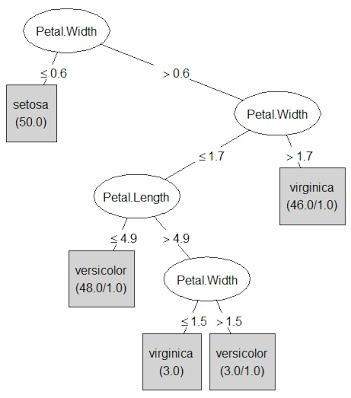
\includegraphics[width=0.5\linewidth]{fig/ml/decision_tree.JPG}
				\caption{A decision tree model built on the Iris dataset \citep{fisher1936use} (source \citet{decisiontree2015}).}
				\label{fig:decision_tree}
			\end{figure}
			\item[Rule induction] Apart from decision trees, various algorithms for inducing rules from training data have been proposed in the literature. The rule induction algorithms aim to minimise the set of rules consisting of training data. Minimising the rule-set ensures generalisation and avoids overfitting \citep{kotsiantis2007supervised}. RIPPER \citep{cohen1995fast}, AQ family \citep{michalski1980learning} and CN2 \citep{clark1989cn2} are some of the more popular rule based learning algorithms.
		\end{description}
		
		 
	\item \textbf{Perceptron based}: Perceptron oriented algorithms are one of the most researched and powerful class of machine learning algorithms. These ML algorithms, as described in the seminal article \citep{rosenblatt1958perceptron}, are inspired by the working principles of the brain, and can be categorised loosely as neuromorphic in nature. Historically, the perceptron based algorithms are divided into two sub categories:
		\begin{description}
			\item[Single layer perceptron] A single layer perceptron model consists of a set of computational neurons (perceptrons) arranged in a single layer and fully connected to the input data $\mathbf{x}$ by connectors with weight $\mathbf{w}$. These networks were equipped to solve a binary classification problem ($\mathbf{y}:={-1, 1}$). The neurons compute weighed sum $\displaystyle \sum_i w_i\cdot x_i$ of the input data, and is passed through an adjustable threshold gate to output $-1$ or $1$. In the ADALINE model the weighed sum is further passed through an activation function \citep{widrow199030}. \figurename \ref{fig:adaline} shows the architecture of the ADALINE network. The most prevalent method of learning the patterns is by running multiple iterations of the training data and adjusting the connection weights $\mathbf{w}$ until the output matches ground truth. Some of the well known learning algorithms for single layer perceptron are described in \citep{littlestone1994weighted, freund1999large}. Despite its computational ability to solve linearly separable binary output problems as shown in \figurename \ref{fig:lin_sep}, these ML algorithms cannot solve problems of non-linearly separable variety, such as, the XOR problem \citep{minsky1969perceptrons}. 
			
			\begin{figure}
			\centering
				\subfloat[Adaptive Linear Elements (ADALINE)]{\label{fig:adaline}
					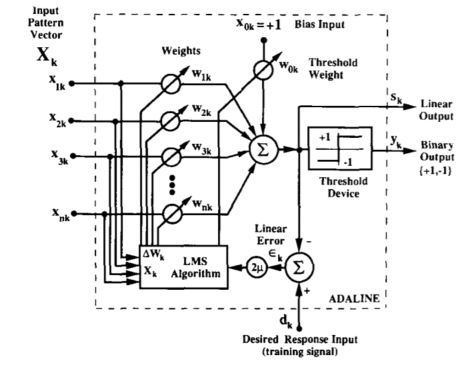
\includegraphics[width=0.45\textwidth]{fig/ml/adaline.JPG}}\hfill
				\subfloat[Example of a linearly separable problem.]{\label{fig:lin_sep}
					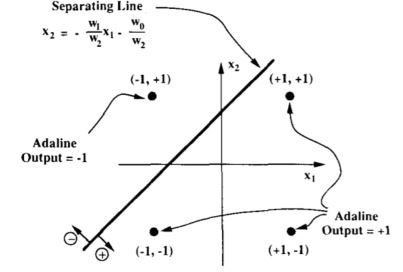
\includegraphics[width=0.45\textwidth]{fig/ml/linearly_separable.JPG}}				
				\caption{The ADALINE single layer perceptron model and an example of linearly separable problem (source \citet{widrow199030}).}			
				\label{fig:adaline_lin_sep}
			\end{figure}
			
			\item[Multi layer perceptron] MLP models are extended from the earlier perceptrons. It is defined as a fully connected feed-forward ANN having multiple layers of nodes arranged as a directed graph. The layers are segregated into three classes: input units, hidden and output units. The hidden elements of MLP possess non-linear activation functions and can distinguish non-linearly separable data. 
			\figurename \ref{fig:mlp} shows an example of an MLP model. The feed-forward MLP networks are trained usually using some variant of the gradient based backpropagation algorithm \citep{rumelhart1988learning}, which optimise the output by minimising the network prediction error by backpropagation of the error. It must be noted that due to the gradient descent-based approach of the learning algorithm, these networks require the activation functions to be fully differentiable and the input data to be in a continuous space. Genetic algorithms have also been used to train the weights of neural networks \citep{siddique2001training} and to find the architecture of neural networks \citep{yen2000hierarchical}. There are also Bayesian methods in existence which attempt to train neural networks \citep{vivarelli2001comparing}. 
			
			\begin{figure}
				\centering
				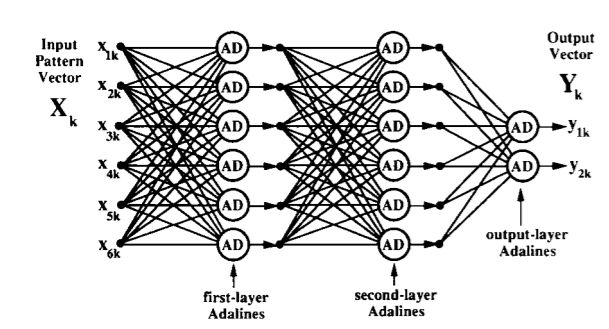
\includegraphics[scale=0.72]{fig/ml/mlp.JPG}
				\caption{A fully connected feed-forward multi layer perceptron model (source \citet{widrow199030}).}
				\label{fig:mlp}
			\end{figure}
		\end{description}  
	\item \textbf{Support vector machines}: SVM is one of the most recent and widely used supervised ML algorithm introduced by \citet{cortes1995support}. It was developed to solve binary classification problems using linear hyperplanes. SVM revolves around the idea of a margin that maximally separates two data classes around a hyperplane (see \figurename \ref{fig:svm_margin}). For linearly separable training data, the tuple $\displaystyle (\mathbf{w},b)$ exists such that:
	\begin{equation}
		\mathbf{w^Tx_i}+b\ge 1\ \forall x_i\in P
	\end{equation}
	\begin{equation}
	\mathbf{w^Tx_i+b\le -1\ \forall x_i\in N}
	\end{equation}
	
	The black and white dots represent the positive class P and negative class N, respectively. The decision rule is given by:
	\begin{equation}
		f_{w,b}(x):=sgn(\mathbf{w^Tx_i}+b)
	\end{equation}
	
	\begin{figure}
		\centering
		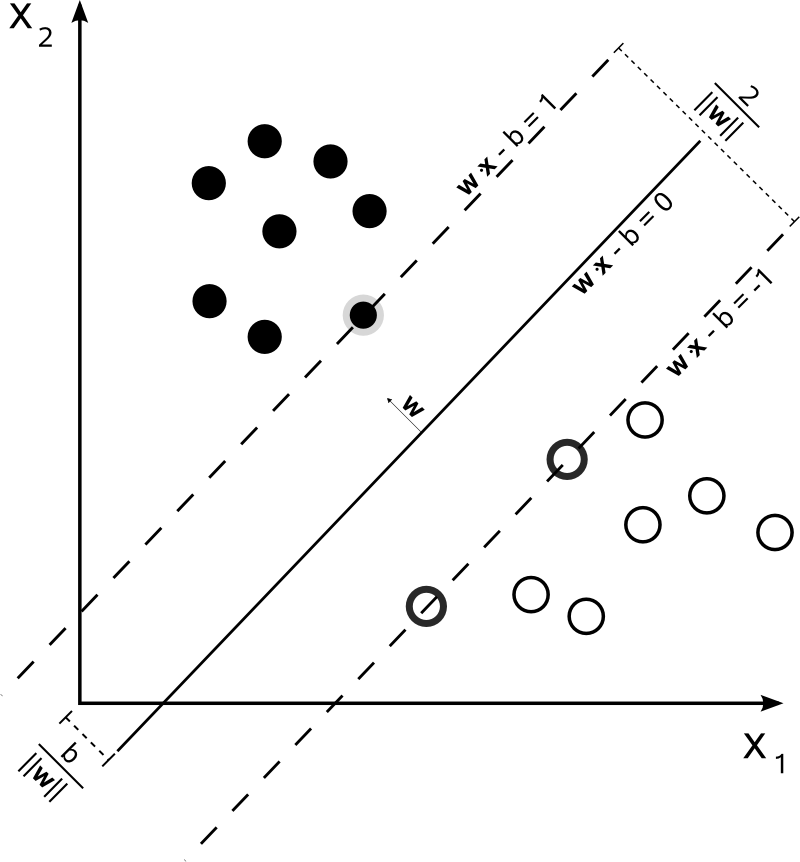
\includegraphics[scale=0.2]{fig/ml/svm_margin.JPG}
		\caption{Maximum-margin hyperplane and margins for an SVM trained with samples having two features from two classes (source \citet{cortes1995support}).}
		\label{fig:svm_margin}
	\end{figure}  
	
	 An optimum separating hyperplane can be found by minimising the squared norm of the separating hyperplane. The minimisation can be set up as a convex quadratic programming (QP) problem:   
	 \begin{equation}
		\begin{matrix}
		\min_{w,b} & \mathbf{\Phi(w):=\frac{1}{2}||w||^2}\\
		\textrm{s.t.} & \mathbf{y_i(w^Tx_i+b)\ge 1}, i=1,\cdots,l \\			 		 
		\end{matrix}
	 \end{equation}
	 For linearly separable data, at the end of the optimally separating hyperplane search, data points lying on its margin are known as support vector points. This hard margin solution is later modified \citep{veropoulos1999controlling} to accommodate misclassification of the training samples.  
	 
	 To overcome the issue of non-linearly separable problems, non-linear SVM is introduced by applying the kernel approach to find maximum margin hyperplanes. The kernel function transforms the given data space in a higher dimensional space in the hope of achieving linear hyperplane in a higher dimension that can separate the classes. There are numerous transformation kernels existing in the literature including:
	  \begin{itemize}
		  \item linear: $K(x_i,x_j)=x_ix_j$
		  \item polynomial: $K(x_i,x_j)=(\gamma x_ix_j+c)^d$
		  \item RBF: $K(x_i,x_j)=\exp(-\gamma|x_ix_j|^2)$
		  \item sigmoid: $K(x_i,x_j)=\tanh(\gamma x_ix_j +c)$
	  \end{itemize}
	  The kernel function represents the dot product of the input data points mapped into higher dimensional feature space. Some of the known disadvantages of SVM are the high computational complexity of the quadratic programming based training phase \citep{horvath2003cmac} and sensitivity to overfitting the model selection criteria in kernel models \citep{cawley2010over}.

\end{enumerate}  


The brief review presented in this chapter are very general and touches upon the two broad strands of research the studies in this thesis belongs to. Chapters \ref{chap:snn} and \ref{chap:neucube} further reviews and delves into the nitty-gritties of computational neuron and network of such neurons as a basis of the main studies presented in Chapters \ref{chap:large_snn}, \ref{chap:encoding} and \ref{chap:multimodal}. Further, literature reviews are also performed locally in the context of the topics.
  





   
